\documentclass[a4paper, 12pt]{article}
\usepackage[utf8]{inputenc}
\usepackage[english,russian]{babel}
\usepackage[warn]{mathtext}
\usepackage{graphicx}
\usepackage{float}
\usepackage{multirow}
\restylefloat{table}
\usepackage{amsmath}
\usepackage{floatflt}
\usepackage[T2A]{fontenc}
\usepackage[left=20mm, top=20mm, right=20mm, bottom=20mm, footskip=10mm]{geometry}
\usepackage{amssymb}

\tolerance 1414
\hbadness 1414
\emergencystretch 1.5em
\hfuzz 0.3pt        % размер максимального переполнения без warning'a
\widowpenalty=10000 % запрещает одиночную строку абзаца в начале страницы
\vfuzz \hfuzz
\raggedbottom       % если на странице мало содержимого, добавить пустое место в конце, а не в середине страницы



\begin{document}

\begin{titlepage}
	\centering
	\vspace{5cm}
	{\scshape\LARGE московский физико-технический институт (национальный исследовательский университет) \par}
	\vspace{6cm}
	{\scshape\Large Лабораторная работа 4.3.6 \par}
	{\huge\bfseries Саморепродукция \par}
	\vspace{1cm}
	\vfill
\begin{flushright}
	{\large Б03-102}\par
	\vspace{0.3cm}
	{\LARGE Куланов Александр}
\end{flushright}
	

	\vfill


	Долгопрудный, 2023 г.
\end{titlepage}

\begin{itemize}
	\item \textbf{Цель работы:} изучение явления саморепродукции и применение его к измерению параметров периодических структур
    \item \textbf{В работе используются:} лазер, кассета с сетками, мира, короткофокусная линза с микрометрическим винтом, экран, линейка
\end{itemize}

\section{Экспериментальная установка}

\begin{figure}[H]
    \centering
    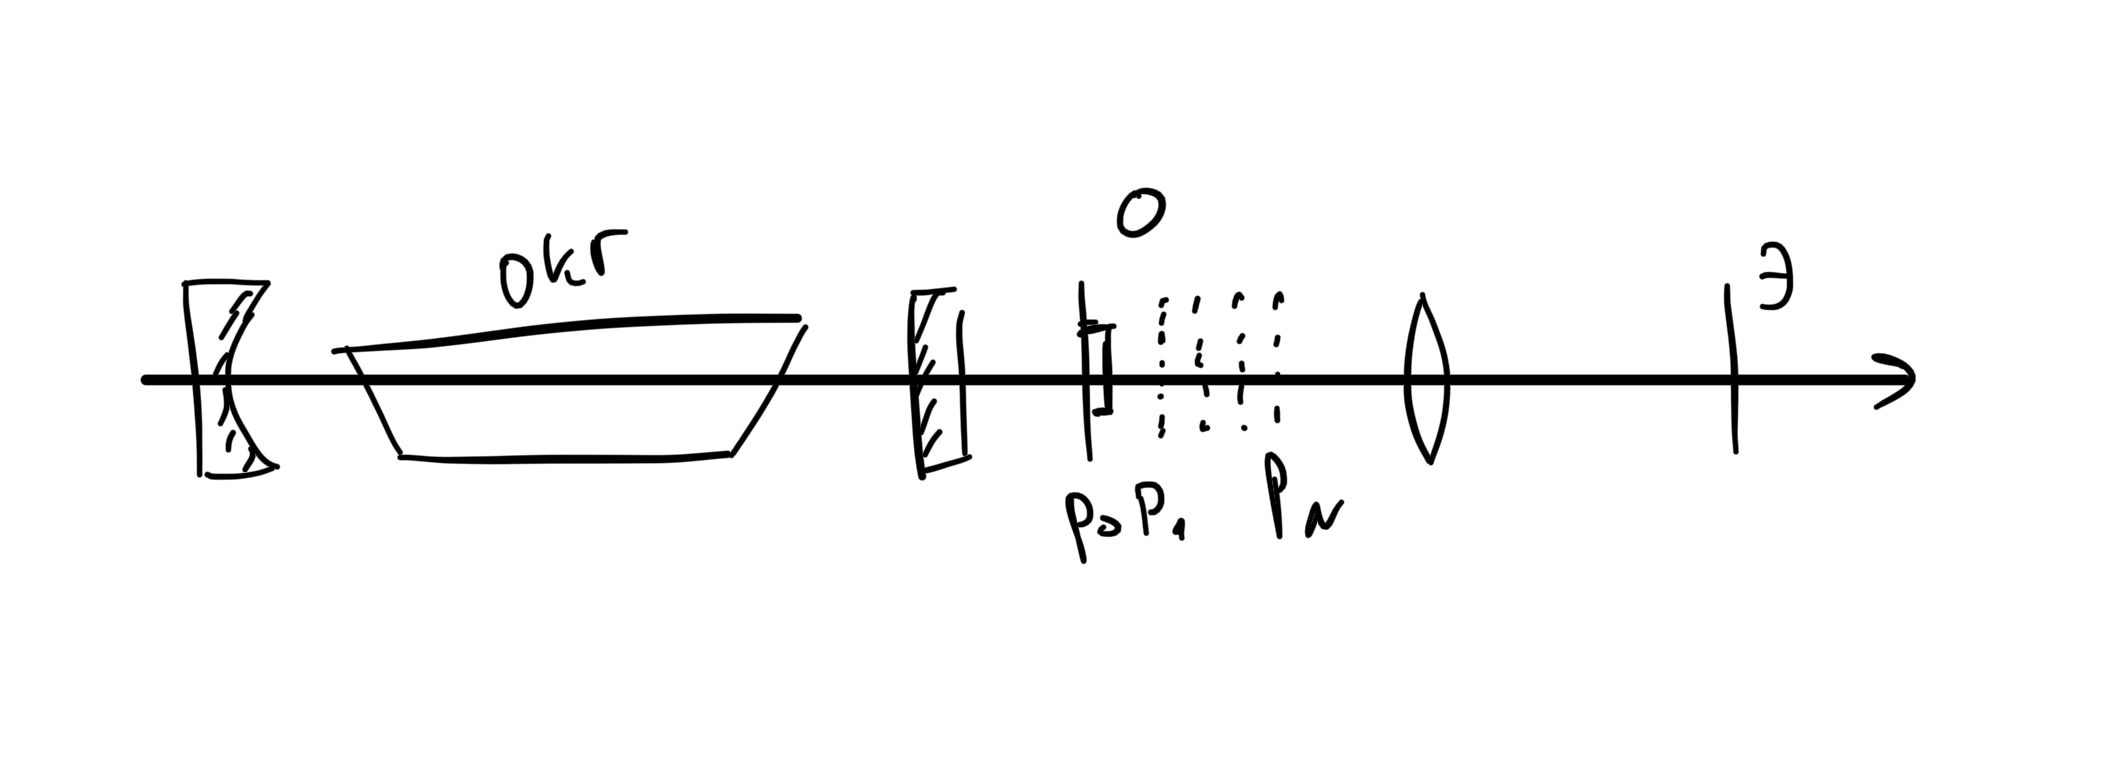
\includegraphics[width=1\textwidth]{set.jpg}
    \caption{Экспериментальная установка}
    \label{fig:set}
\end{figure}

ОКГ --- гелий-неоновый лазер, 0 --- двумерная решетка, PN --- плоскости, где наблюдаются репродуцированные изображения, Л --- короткофокусная линза, Э --- экран для наблюдения изображения объекта

За плоскостью P0 периодически по z возникают изображения объекта, которые с помощью линзы Л можно поочередно проецировать на экран, установленный в плоскости Э.
Если убрать линзу, то на экране наблюдается картина дифракции луча на периодическом объекте.

Экран устанавливается достаточно далеко от объекта, так что продифрагированные лучи, соответствующие различным порядкам дифракции, разделяются.

Измерив расстояние от объекта до экрана, можно определить $\sin \varphi$ и $d$





\end{document}